\title{ \vspace{5cm}
\begin{Huge}
\textsc{Algorithms and Computability
Project Report}\\ 
\end{Huge}
\begin{Large}
\textsc{The 2D Bin Packing Problem}
\end{Large}
\vspace{1cm}}
\author{
Igor Sa\l uch\\
Jianhao Luo
}
\date{}

\documentclass[12pt]{article}
\usepackage[margin=1in]{geometry}
\usepackage{graphicx}
\graphicspath{ {img/} }
\usepackage{float}
\usepackage{csquotes}
\usepackage{hyperref}
\usepackage{listings}
\usepackage{xcolor}
 
\definecolor{codegreen}{rgb}{0,0.6,0}
\definecolor{codegray}{rgb}{0.5,0.5,0.5}
\definecolor{codepurple}{rgb}{0.58,0,0.82}
\definecolor{backcolour}{rgb}{0.95,0.95,0.92}
 
\lstdefinestyle{mystyle}{
    backgroundcolor=\color{backcolour},   
    commentstyle=\color{codegreen},
    keywordstyle=\color{magenta},
    numberstyle=\tiny\color{codegray},
    stringstyle=\color{codepurple},
    basicstyle=\ttfamily\footnotesize,
    breakatwhitespace=false,         
    breaklines=true,                 
    captionpos=b,                    
    keepspaces=true,                 
    numbers=left,                    
    numbersep=5pt,                  
    showspaces=false,                
    showstringspaces=false,
    showtabs=false,                  
    tabsize=2
}
 
\lstset{style=mystyle}
\begin{document}
\begin{titlepage}
\maketitle
\vfill
{\centering \large November 19, 2019 \par}
\pagenumbering{gobble}
\end{titlepage}
\newpage
\pagenumbering{arabic}

% TODO consider rotations (maybe rotate before discarding)
% TODO add proof of correctness
% TODO show initial list of rectangles on the visualistion
% TODO show rectangle values of the visualisation


\section{Introduction}
It is a common problem of trying to pack a lot of items in limited space.
For example, truck loaders deal with such problem every day --
how to load a truck as efficiently as possible,
but without overloading the vehicle.
It is also sometimes called ``a thief problem'', where a burglar tries
to pack as many items as possible into their backpack.

In computer science, we also deal with this problem very often.
Packing virtual machines on a server with limited memory is a problem set
on completely different kind of resources,
but still solved using the same principles.
For example, we want to present the user their photos on the thumbnail view,
without cropping, while retaining the sizes (or at least ratios).

\section{Problem description}
The \textit{bin packing problem} is an combinational optimization problem.
According to Wikipedia\cite{wikibinpacking},
\begin{displayquote}
\textelp{} \textit{items of different volumes must be packed into a finite number of
bins or containers each of a fixed given volume in a way that minimizes the
number of bins used.}
\end{displayquote}
The problem has many variations,
it arises in various places where space resources are limited and there is a
need to find the best packing.

In our case, the limited resource is a \textbf{two dimensional space}.
We have a set of rectangles (blocks),
each with its own \textbf{height} and \textbf{width}.
In addition, each block has it's own \textbf{value}.
We want to score as much value points as we can,
by fitting in a fixed space as much blocks (of the best values),
as we can.

\newpage
\section{Solution}
\subsection{Solution description}
Before diving into details, let us start with a brief,
step-by-step description of the algorithm.

\begin{enumerate}
  \item Find all permutations of the input set,
    including all rotations.
  \item For each permutation of the input set, do the following:
  \begin{enumerate}
    \item Put the first item from the list in the top left corner,
    \item Split the remaining space into 2 rectangles, one on the right
      to the first item, another below,
    \item Repeat steps 2 and 3 recursively in the form of a binary tree
      until there is no more space left.
    \item Save the value score.
  \end{enumerate}
  \item Compare scores and pick the best packing. 
\end{enumerate}

\subsubsection{Permutation}
First we permutate and rotate our input set in order to get
all possible packings for all rotations.
Then we can proceed to find the best fit for each permutation.

\subsubsection{Placing the block}
This step is quite simple -- we need to put the block somewhere,
and one of the corners would let us have a two-rectangle split for the next step.
Top left corner is an arbitrary choice -- it can be any other corner as long
as we are consistent with our choice.
We store all whitespace rectangles in a binary tree.

\subsubsection{Splitting the remaining space}
We divide the remaining whitespace in order to allow recursion.
Each smaller part can be treated as a new rectangle
for fitting blocks from our queue.
\begin{figure}[H]
  \centering
	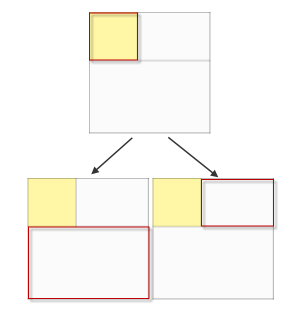
\includegraphics[width=.5\textwidth]{split}
  \caption{Visualisation of splitting the space and binary tree creation}
  \label{fig:split}
\end{figure}

\subsubsection{Recursion}
Finally, we do the same thing again for each new item to pack,
and for the each smaller whitespace rectangle.
There is one caveat, though -- we do it in a form of binary tree.
It simply means that we traverse our tree to find the smallest free space
in which our rectangle would fit.
If there is no such space, we discard our block and proceed to the next one.

\subsubsection{Saving and comparing scores}
After calculating all packings for each permutation,
we can pick one of the best value.

\newpage
\subsection{Solution pseudocode}
\begin{lstlisting}[language=Python, caption=Python-style pseudocode]
# defines the rectangle we want to pack
class Block:
  width: int
  height: int
  value: int  # the price of the rectangle
  fit: Node or None


# defines the container and subcontainer
class Node:
  right: Node
  down: Node
  position.x: int
  position.y: int
  width: int
  height: int
  used: bool

  # Node Methods:
  def fit(self, blocks):
    for each block in the blocks:
      # try to find a node that suits current block
      node = self.findNode(block.w, block.h) 
      if find a node: 
        # pack and split the Node
        block.fit = node.splitNode(block.w, block.h) 

  def findNode(self, w, h):
    # if self is already occupied, 
    # we look for its neighbours recursively
    if self.used: 
      return self.right.findNode(w, h) or self.down.findNode(w, h)
    # if current fits then we return current Node
    else if self.width >= w and self.height >= h: 
      return self
    else:
      # Nothings fits for the block
      return 0 

  def splitNode(self):
    # now the node is used
    self.used = True
    self.right = Node(self.x+w, self.y, self.width-y, h)
    self.down = Node(self.x, self.y+h, self.width, self.height-h)
    return self


def get_all_permutations(input):
  output = []
  rotated = get_all_rotations(input)
  for rotated in rotations:
    output.append(
      itertools.permutations(rotated)  # built-in permutation function
    )

def getValueBlocks(block_list, out_list):
    out_list.clear()
    S=0
    for block in block_list:
        if not block.fit is None:
            out_list.append((block.fit.x, block.fit.y, block.w, block.h))
            S+=block.value
    return S

def main():
  input = read_input_file()  # read the input file
  permutations = get_all_permutations(input)
  for permutation in permutations:
    root = Node(
      permutation[0], permutation[1], permutation[2], permutation[3]
    )
    root.fit(block_list_t)
    out_list_t = []
    value = getValueBlocks(block_list_t, out_list_t)
    if value>value_max:
        out_list=out_list_t
        value_max=value

  display_packing(out_list, value_max)

\end{lstlisting}

\subsection{Pseudocode description}
The \texttt{Node.insert} function traverses the tree looking for a place
to insert the block.
It returns the node the block can be placed into or \texttt{None} to say
it could not fit.

The code that calls \texttt{Node.insert} can then use the rectangle
from the returned node to figure out where to place the block in the space,
then update the node's \texttt{block\_id} to use as a handle for future use.

\subsection{Time complexity calculation}

\subsubsection{Finding and splitting}
Each time it traverses to find a suitable node is  Depth First Traversal in binary search tree.
Imagine we have N-1 blocks already packed, we want to pack the N th rectangle
The worst case of the nodes number will be $N+1$
So the time complexity of the worst finding is $\mathcal{O}(N)$
To sum it up from 1 to $N$
The time complexity will be $\mathcal{O}(N^2)$
(we assume splitting is a constant timing consume also) 
So the worst case of finding and spliting for $N$ blocks
will be $\mathcal{O}(N^2)$

\subsubsection{Permutations and getting values}
For $N$ blocks we have $N!$ permutations, for each permutation the worst
finding and splitting time complexity will be $\mathcal{O}(N^2)$
Our project time complexity will be
$$T_C=\mathcal{O}(N^2*N!)$$

\section{Conclusion}
Although the algorithm is quite \textit{brute-force} in some aspects,
which may be especially cumbersome on larger input,
it provides very good results, aside from
being simple and easy to understand.

\newpage
\begin{thebibliography}{9}
\bibitem{wikibinpacking}
	\url{https://en.wikipedia.org/wiki/Bin_packing_problem}
\end{thebibliography}

\end{document}
